


\subsection{Code structure}

\subsubsection{Overview of the classes}
The code provided for the project were made up of several classes, each with different roles. To a large extent there is a hierarchy in the classes, with  \textit{main} being on the top. From this class all main processes are initiated, initial conditions are determined, and the integration loop is run. However, it is the class \textit{atom} that facilitate the object in which to store information about each atom in the calculation. Under follows a quick overview of each class and the main purpose of it. 
		
		\begin{itemize}

			\item \textit{system}:\\
				Contains all the information about the system. Creates a system of atom-instances in a fcc lattice. It also contains the integration function, linking the system to \textit{VelocityVerlet}. In addition, functions that are relevant to the behaviour of the system, like applying periodic BC's and calculation of forces are found here. 
				
			\item \textit{atom}:	\\
				Contains information about each atom in the simulation, like starting position,  position, velocity and force experienced by each atom. Is mainly a class to store information about each atom, but also contains a function to calculate the initial velocity distribution.
			
			\item \textit{VelocityVerlet}:\\
					Contains simply the velocity verlet algorithm (per timestep). Takes the entire system class as an input variable and updates position, velocity and force on each atom in the system. Uses functions from \textit{system} in order to update forces and utilize periodic BC's. 
						
			\item \textit{LennardJones}:\\
				When calling the \textit{calculateForces} function in \textit{system}, it links to this object. Updates forces on each atom in the system and the total potential, through the Lennard Jones potential.
				
			\item \textit{statisticssampler}:\\
				Collect information about the system, like kinetic and potential energy, instantaneous temperature. In addition, also contains a unit test checking energy convergence. 
			
			\item 	\textit{vec3}:\\
				Defining the behaviour of every $ 3\times 1 $ vector utilized in the program.  Also contains functions to calculate length of  \textit{vec3} objects, cross products, nullifying a \textit{vec3}  instance. Every vector in the code is a \textit{vec3} instance.
				
			\item \textit{unitconverter}:\\
				Contains information about  constants and units used in the program, in addition to functions converting values between MD-units and SI units. 
			

			\item \textit{io}:\\
				Framework to create and store information to a $ .xyz $ file. 
			\item 	\textit{random.h}:	\\
				Header file containing a selection of functions from the c++ library \textit{random} and \textit{ctime}.
		\end{itemize}


\subsubsection{Program flow}

\begin{figure}[H]
	\centering
	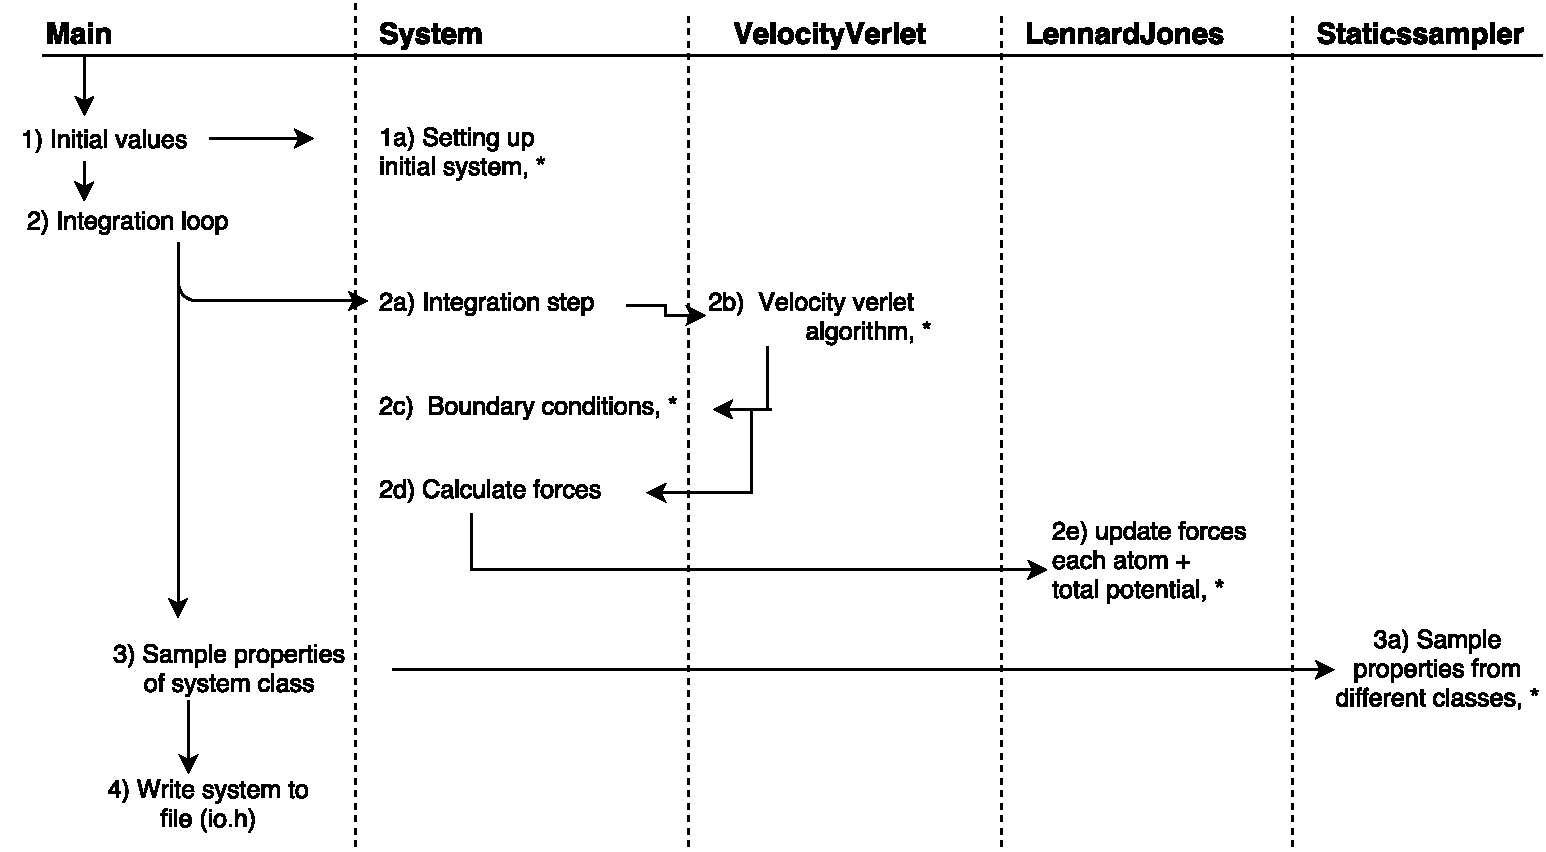
\includegraphics[width=1\linewidth]{../figures/klasser_proj5}
	\caption{Simplified flow chart of the code structure. * indicates that the Atom class was used, see the discussion below}
	\label{fig:klasserproj5}
\end{figure}

Figure \ref{fig:klasserproj5} illustrates the work flow in the code somewhat simplified. Due to the amount of classes in this project, every time the \textit{atom} class is called is marked by *. As  \textit{system} contains several atoms, each time \textit{atom} is called is by a loop over all the atoms in \textit{system}, updating i.e. the position. To some extent, all the classes can be viewed as a blackbox, with \textit{main} controlling the sequence and what is being performed. 

Step 1)specifies the initial values, like temperature and number of unit cells, sending them to step 1a, which creates the fcc lattice as specified by main. In addition, it also creates instances of \textit{io} and \textit{staticssampler} and initialize  the output files.  It also creates the specified amount of \textit{atom}-instances. In order to integrate the system through time, a time loop is performed in \textit{main}. However, each integration step is then micromanaged by \textit{system} through an instance of \textit{VelocityVerlet}, which does the actual integration over every instance of \textit{atom} in \textit{system}. Through the instance "system" the periodic boundary conditions are applied and forces are calculated, see snippet below. 

\lstset{language=C++,
	numbers=left,
	stepnumber=1,
	basicstyle=\ttfamily,
	keywordstyle=\color{blue}\ttfamily,
	stringstyle=\color{red}\ttfamily,
	commentstyle=\color{green}\ttfamily,
	morecomment=[l][\color{magenta}]{\#}
	    showstringspaces=true,
	tabsize=1,
	}
\begin{lstlisting}[caption = {Snippet showing the main part of velocity verlet algorithm as applied in \textit{VelocityVerlet}}, label = {listing}]
	double dthalf = dt*0.5;
	for(Atom *atom : system.atoms()) {
		atom->velocity += dthalf*atom->force/(atom->mass());
		atom->position += atom->velocity*dt; 
		//atom->position += atom->velocity*dt/atom->mass();
	}
	system.applyPeriodicBoundaryConditions();
	system.calculateForces();
	
	for(Atom *atom : system.atoms()) {
		atom->velocity += dthalf*atom->force/(atom->mass());
		}

\end{lstlisting}		
 
 The sampling of properties are done in step 3, by applying the "sample" function in \textit{Staticssampler}, 3a. This function updates the private variables of  \textit{Staticssampler}, describing properties like temperature and kinetic energy. This is done by calling several specific \textit{Staticssampler} - functions sampling each property individually. The last step, step 4, writes .xyz-file through the \textit{io} instance "movie" in \textit{main}. In addition, the information stored in \textit{Staticssampler} is saved in a separate output file. This should be done in \textit{io} for the most logical flow, but we found it simplest to do this through \textit{Staticssampler}. 
  



\subsection{Computational details}

This project used the velocity verlet algorithm in order to integrate the partial differential equations which arises from the newtons second law. 	The velocity Verlet can be derived from a  Taylor expansion around the position $ r(t+\Delta t) $. However, for the velocity there exist a similar Taylor series: $  v_{i+1} = v_i + h\dot{v}_i + \frac{h}{2} \ddot{v}_i + O(h^3)$. Unfortunately, there is no expression for $ \ddot{v}_i $, but it can be approximated by $ h\ddot{v}_i \simeq \dot{v}_{i+1}-\dot{v}_i$. Adding this to the expression for $ v_{i+1} $ and doing some simple algebra one get the final expression for the velocity:

\begin{equation}
v_{i+1} = v_i +  \frac{h}{2} \left(\dot{v}_{i+1}+\dot{v}_i\right)+ O(h^3) \label{eq:vel_verlet}
\end{equation}

Looking a bit closer at equation \ref{eq:vel_verlet}, there is a immediate problem. In order to calculate $ v_{i+1} $ one need to already know $ v_{i+1} $. This problem can be solved by updating the velocity in two steps, which gives the following algorithm:

\begin{align}
v_{i+\frac{1}{2}} &= v_i + \frac{h}{2} a_i\\
x_{i+1} &= x_i + v_{i+\frac{1}{2}}\\
a_{i+1} &= \frac{F_{i+1}}{m}\\
v_{i+1} &=v_{i+\frac{1}{2}}. + \frac{h}{2} a_{i+1}
\end{align} 






\subsection{Bugs and unit tests}

As the structure  of the program was provided, a large array of unit tests were not necessary. However, two simple test became very useful. The first, checking that the total momentum was set to 0 provided useful input, as the initial version of "removeTotalMomentum" did not take the changing unit cell size into account. Secondly, the unit test for the conservation of energy revealed several mistakes. One example of this is that we counted the potential energy per atom in interacting pair, instead of each pair. A more serious bug were found in \textit{velocityVerlet} through this unit test. Line 5 in snippet \ref{listing} shows the original, first position update in the algorithm. Here the velocity of each atom is divided by the atom mass, which has no place in the relationship $ \dv{v}{t} = x(t) $. Most likely this is due to a copy and paste error of the line above, simply substituting the force with velocity. 

\subsubsection{Units} \label{sec:units}

In order to avoid round off errors and produce results with direct physical meaning, a specific set of units were used. These molecular dynamics units are presented in the project description, and are:

\begin{align}
\text{1 unit of mass } &= 1 \text{ a.m.u} = 1.661\times 10^{-27}\mathrm{kg},\\
\text{1 unit of length } &= 1.0 \text{ \AA} \\
\text{1 unit of energy } &= 1.651\times 10^{-21}\mathrm{J},\\
\text{1 unit of temperature} &= 119.735\mathrm{K}.\\
\text{1 unit of Force}  &= \\
\text{1 unit of Pressure}  &= 
\end{align}





